% Artigo técnico do Projeto Final (Tendências em Ciência da Computação).
% Formato SBC: no Overleaf, abra o modelo "SBC Conferences Template" e substitua o
% arquivo principal por este, enviando também referencias.bib e a pasta figuras/.
% Sem o sbc-template.sty, o documento compila com uma formatação equivalente
% (A4, Times 12 pt, margens de 3 cm), útil para revisão local.
\documentclass[12pt]{article}

\makeatletter
\IfFileExists{sbc-template.sty}{%
  \usepackage{sbc-template}%
}{%
  \usepackage[a4paper,top=3.5cm,bottom=2.5cm,left=3cm,right=3cm]{geometry}%
  \usepackage{times}%
  \newcommand{\address}[1]{\gdef\@address{#1}}%
  \newenvironment{resumo}{\begin{center}\small\bfseries Resumo\end{center}\begin{quote}\small\itshape}{\end{quote}}%
  \renewcommand{\maketitle}{\begin{center}{\Large\bfseries\@title\par}\vspace{1em}{\@author\par}\vspace{0.5em}{\small\@address\par}\end{center}\vspace{1em}}%
}
\makeatother
\usepackage[T1]{fontenc}
\usepackage[utf8]{inputenc}
\usepackage[brazil]{babel}
\usepackage{graphicx}
\usepackage{url}
\usepackage{booktabs}
\usepackage{amsmath}

\sloppy

\title{GraphRAG e KAG para Consulta a Normas Acadêmicas:\\
Recuperação Híbrida sobre Grafo de Conhecimento em Neo4j}

% Preencha com os integrantes do grupo e a instituição.
\author{Integrante 1\inst{1}, Integrante 2\inst{1}, Integrante 3\inst{1}, Integrante 4\inst{1}}

\address{Curso de Bacharelado em Ciência da Computação -- Instituição\\
  Cidade -- UF -- Brasil
  \email{\{integrante1,integrante2\}@instituicao.edu.br}
}

\providecommand{\inst}[1]{\textsuperscript{#1}}
\providecommand{\email}[1]{\\\texttt{#1}}

\begin{document}

\maketitle

\begin{abstract}
Large Language Models hallucinate and struggle with multi-hop questions, which limits
their use for consulting academic regulations. We present an open-source GraphRAG/KAG
prototype for higher education that combines a Labeled Property Graph in Neo4j, an
LLM-based text-to-graph pipeline with entity resolution and semantic type constraints,
and a hybrid retriever that fuses vector and lexical search, explores multi-hop graph
neighborhoods ranked by PageRank and Leiden communities, and runs validated read-only
Text2Cypher queries. Answers must cite numbered evidence, citations are verified, and a
transparent confidence level is shown together with an interactive context subgraph.
On 35 questions derived from a synthetic gold graph and a 3B-parameter local model, the
hybrid approach raised answer coverage from 0.76 to 0.89 (from 0.35 to 0.72 on questions
with three or more hops), cut answers containing unexpected entities from 55\% to 34\%,
and raised valid citations from 48\% to 99\%, compared with a vector-only baseline.
\end{abstract}

\begin{resumo}
Modelos de Linguagem de Grande Porte alucinam e falham em perguntas que exigem
raciocínio em múltiplos saltos, o que limita seu uso na consulta a normas acadêmicas.
Este trabalho apresenta um protótipo aberto de GraphRAG/KAG para a educação superior que
combina um grafo de propriedades rotulado no Neo4j, um pipeline de extração de
entidades e relações por LLM com resolução de entidades e restrições semânticas de
tipos, e um recuperador híbrido que funde buscas vetorial e lexical, percorre vizinhanças
multi-hop ordenadas por PageRank e comunidades Leiden e executa consultas Cypher geradas
pelo LLM, validadas e somente de leitura. As respostas citam evidências numeradas, as
citações são verificadas e um nível de confiança transparente é exibido com o subgrafo
de contexto interativo. Em 35 perguntas derivadas de um grafo-gabarito sintético, com um
modelo local de 3 bilhões de parâmetros, a abordagem híbrida elevou a cobertura das
respostas de 0,76 para 0,89 em relação a um baseline somente vetorial (de 0,35 para 0,72
nas perguntas de três ou mais saltos), reduziu de 55\% para 34\% as respostas com
entidades não esperadas e elevou as citações válidas de 48\% para 99\%.
\end{resumo}

\section{Introdução}

A geração aumentada por recuperação (RAG) fundamenta as respostas de um LLM em trechos
recuperados de uma base documental~\cite{lewis2020rag}. Na consulta a normas
acadêmicas, como Projetos Pedagógicos de Curso (PPC) e regulamentos, duas limitações do
RAG vetorial são críticas. A primeira são as \emph{alucinações}: respostas plausíveis sem
apoio nas fontes~\cite{ji2023hallucination}. A segunda é o \emph{raciocínio multi-hop}:
perguntas como ``quais são todos os pré-requisitos, diretos e indiretos, de Grafos de
Conhecimento?'' exigem encadear fatos espalhados em trechos que a similaridade com a
pergunta não recupera juntos.

Abordagens baseadas em grafos de conhecimento, como GraphRAG~\cite{edge2024graphrag,peng2024survey}
e KAG~\cite{liang2024kag}, tornam explícitas as entidades e relações do domínio e permitem
percorrê-las de forma estruturada. Este trabalho, desenvolvido como Projeto Final da
disciplina Tendências em Ciência da Computação, implementa e avalia os quatro pilares da
especificação: (i) pipeline \emph{Text-to-Graph} com resolução de entidades; (ii)
modelagem LPG no Neo4j com constraints e índices; (iii) recuperação híbrida com travessia
multi-hop e algoritmos de grafo; e (iv) interface com visualização do subgrafo e
métricas de rastreabilidade. O código, os dados e os scripts de avaliação estão no
repositório do projeto.

\section{Fundamentação e trabalhos relacionados}

O GraphRAG da Microsoft~\cite{edge2024graphrag} extrai um grafo de entidades de um
corpus, agrupa-o em comunidades com o algoritmo de Leiden~\cite{traag2019leiden} e
resume cada comunidade para responder a perguntas globais. O HippoRAG~\cite{gutierrez2024hipporag}
usa o PageRank personalizado~\cite{page1999pagerank} sobre um grafo de conhecimento como
memória de longo prazo para recuperação multi-hop. O KAG~\cite{liang2024kag} enfatiza
domínios profissionais: alinha conhecimento e trechos de forma bidirecional, aplica
restrições de esquema e decompõe perguntas em formas lógicas executadas sobre o grafo.

Nosso protótipo adota elementos dessas três linhas em escala didática. Do GraphRAG vêm
as comunidades Leiden. Do HippoRAG, o PageRank para priorizar contexto. Do KAG, as
restrições semânticas (allowlist de rótulos e relações e assinatura de tipos), o
planejamento das relações a partir da pergunta e as cadeias lógicas entregues prontas
ao LLM. Não implementamos o raciocínio simbólico formal do KAG.

\section{Arquitetura e modelagem}

O sistema é orquestrado por Docker Compose: Neo4j 5.26 com o plugin Graph Data Science,
Ollama com os modelos \texttt{llama3.2:3b} (geração e extração) e \texttt{nomic-embed-text}
(embeddings de 768 dimensões~\cite{nussbaum2024nomic}) e uma interface Streamlit.

\subsection{Modelo LPG}

Seguimos o modelo de grafo de propriedades rotulado~\cite{robinson2015graphdb}. Toda
entidade de domínio tem o rótulo \texttt{Entity} e um rótulo específico
(\texttt{Disciplina}, \texttt{Curso}, \texttt{MatrizCurricular}, \texttt{Competencia},
\texttt{Regulamento}, \texttt{Artigo}, entre outros) e as propriedades \texttt{id}
canônico, \texttt{name}, \texttt{aliases}, \texttt{embedding}, \texttt{pagerank} e
\texttt{community}. Os documentos (\texttt{Document}) são divididos em trechos
(\texttt{Chunk}) com texto, localização e embedding, ligados por \texttt{FROM\_DOCUMENT}
e às entidades citadas por \texttt{MENTIONS}. As relações de domínio (\texttt{EXIGE},
\texttt{INCLUI}, \texttt{EQUIVALE\_A}, \texttt{DESENVOLVE}, \texttt{DEFINE}, entre
outras) guardam a \textbf{procedência}: a frase literal que as sustenta
(\texttt{evidence}), o trecho de origem (\texttt{evidence\_id}) e o tipo de fonte.

O esquema define constraints de unicidade de \texttt{id} em \texttt{Entity},
\texttt{Chunk} e \texttt{Document}; índices RANGE, sucessores do BTree no Neo4j 5, em
nome, rótulo, comunidade e PageRank das entidades e em versão e localização dos
documentos; índices fulltext com o analisador \texttt{brazilian}, que radicaliza o
português; e índices vetoriais de cosseno em \texttt{Chunk.embedding} e
\texttt{Entity.embedding}. Uma \textbf{assinatura de tipos} por relação (por exemplo,
\texttt{ADOTA}: \texttt{Curso} $\rightarrow$ \texttt{MatrizCurricular}) é aplicada na
gravação de cada aresta.

\subsection{Dados}

Usamos um corpus sintético de uma universidade fictícia: o PPC 2026 (40 disciplinas
em 8 períodos, com pré-requisitos, competências e ementas), o PPC 2022 (matriz anterior e
tabela de equivalências) e o Regulamento Acadêmico 2026. Um script gera, a partir de uma
única definição, os textos e o \textbf{grafo-gabarito} (75 entidades e 167 relações),
garantindo que cada relação tenha uma frase de evidência literal no corpus. Os dados
sintéticos dão um gabarito exato e reprodutível e evitam questões de privacidade.

\section{Pipeline Text-to-Graph}

Os documentos (PDF, TXT ou Markdown) são divididos em trechos por parágrafo, de até 900
caracteres, repetindo o título da seção. Para cada trecho, o LLM devolve entidades e
relações em JSON restrito por um esquema (saída estruturada do Ollama). O prompt inclui um
glossário de rótulos e um exemplo. São descartados: rótulos e relações fora da allowlist,
nomes que não aparecem no texto, nomes reservados e relações cuja evidência não é um
trecho literal do texto.

A \textbf{resolução de entidades} decide, em cascata e dentro do mesmo rótulo, se a
entidade extraída já existe: mesmo id canônico, alias, sigla com iniciais únicas
(``POO''), similaridade de caracteres ($\geq 90$) e similaridade de embedding
($\geq 0{,}96$ na escala $(1+\cos)/2$ do Neo4j). A calibração mostrou que embeddings
aproximam entidades distintas (``Estruturas de Dados I'' e ``Estruturas de Dados''
obtêm 0,973). Por isso, duas proteções bloqueiam fusões: numerais diferentes e nomes em
que um estende o outro. Se o id já existe com outro rótulo, o rótulo registrado
prevalece; isso evita que um erro de rotulagem do modelo corrompa um nó existente.

\section{Recuperação híbrida e geração fundamentada}

Para cada pergunta, o sistema: (1) liga entidades por menção explícita de nomes e
aliases ou, na falta delas, por busca vetorial e fulltext de entidades; (2) recupera
trechos por busca vetorial e fulltext, fundidos por \emph{Reciprocal Rank
Fusion}~\cite{cormack2009rrf}, e acrescenta os trechos de procedência das relações
recuperadas; (3) escolhe as relações relevantes a partir de palavras da pergunta (por
exemplo, ``pré-requisito'' $\rightarrow$ \texttt{EXIGE}) e expande de 1 a 3 saltos a
partir das âncoras, sem atravessar hubs (grau $> 15$), ordenando por distância e
PageRank; (4) para relações dirigidas, monta \textbf{cadeias completas}, como
\textit{Projeto Integrador $\rightarrow$ Banco de Dados $\rightarrow$ Estruturas de Dados
$\rightarrow$ Algoritmos}, entregando ao LLM o raciocínio multi-hop já resolvido pelo
grafo; (5) acrescenta caminhos mínimos entre âncoras e a comunidade Leiden de cada uma.

O \textbf{Text2Cypher} gera uma consulta a partir do esquema, de exemplos e das
entidades reconhecidas. Antes de executar, uma validação estática recusa escrita,
procedimentos, múltiplas instruções e rótulos ou relações fora da allowlist, e impõe
\texttt{LIMIT}. A execução ocorre em transação de leitura com timeout, então o próprio
Neo4j rejeita qualquer escrita. Em caso de erro, há uma nova tentativa com a mensagem de
erro.

As evidências são numeradas (\texttt{[T\#]} trechos, \texttt{[P\#]} relações e cadeias,
\texttt{[C\#]} linhas do Cypher, \texttt{[G\#]} comunidades) e o LLM deve citá-las. Cada
citação é conferida contra o contexto, e citações inexistentes são sinalizadas. A
\textbf{confiança} combina, com pesos documentados, a fração de citações válidas, a
força da busca vetorial, a cobertura do grafo e o resultado do Cypher. Abstenções são
sempre classificadas como confiança baixa.

\section{Interface e explicabilidade}

A interface Streamlit exibe a resposta, a confiança com seus sinais, a contagem de
citações válidas e o \textbf{subgrafo de contexto interativo} (vis-network): a cor
representa a comunidade, o tamanho o PageRank, uma estrela marca a entidade da pergunta e
uma borda escura as entidades citadas; a frase de evidência aparece no
\emph{tooltip} de cada aresta (Figura~\ref{fig:subgrafo}). Abas mostram as evidências
numeradas, os nós consultados, as consultas Cypher executadas e os trechos usados. É
possível alternar para o modo somente vetorial e comparar as abordagens na própria
interface.

\begin{figure}[ht]
\centering
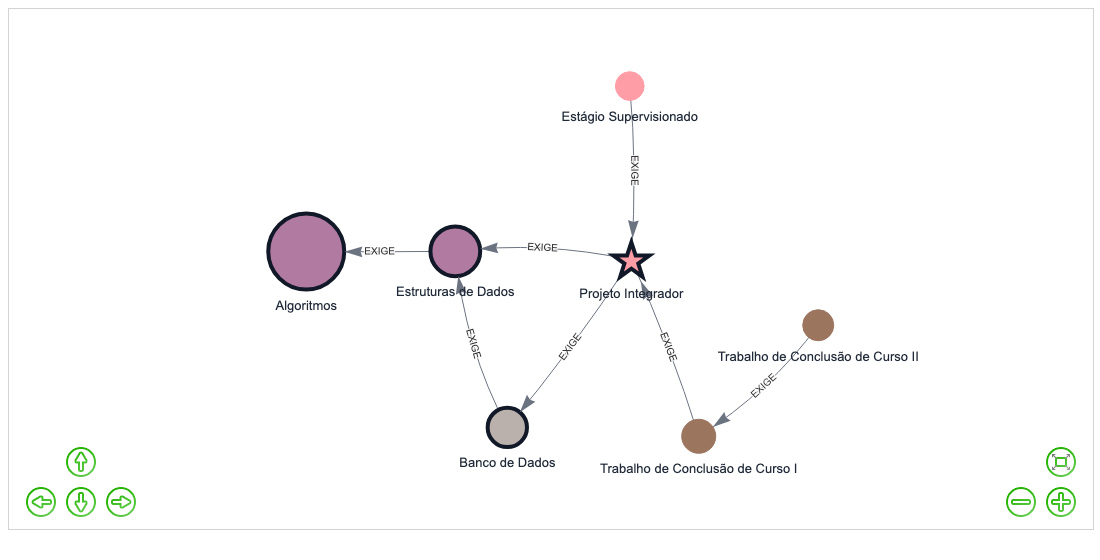
\includegraphics[width=.85\textwidth]{figuras/subgrafo.png}
\caption{Subgrafo de contexto para ``Quais disciplinas antecedem indiretamente Projeto Integrador?''.}
\label{fig:subgrafo}
\end{figure}

\section{Avaliação}
\label{sec:avaliacao}

\subsection{Metodologia}

Um script gera 35 perguntas a partir do grafo-gabarito, de modo que as respostas
esperadas são exatas: 20 de um salto (pré-requisitos diretos, dependentes,
equivalências, competências, matriz, regulamento e fatos textuais), 5 de dois saltos
(por exemplo, o pré-requisito, na Matriz 2022, da disciplina equivalente a Estruturas de
Dados Avançadas), 4 de três a seis saltos (todos os pré-requisitos, diretos e indiretos,
de uma disciplina) e 6 sem resposta no corpus (nota ou decisão individual de estudante,
pessoa não mencionada, disciplina ou matriz inexistente). Cada pergunta é respondida no
modo \textbf{GraphRAG híbrido} e no \textbf{baseline somente vetorial} (6 trechos mais
similares), com o mesmo modelo (\texttt{llama3.2:3b}, temperatura 0, em CPU) e o mesmo
prompt de geração.

Medimos: a \emph{cobertura do contexto} (fração das entidades e fatos esperados presentes
nas evidências); a \emph{cobertura da resposta} (fração citada na resposta); a
\emph{precisão de entidades} (entidades do domínio citadas que pertencem à resposta,
desconsiderando as da pergunta); as \emph{respostas exatas} (cobertura 1 sem entidades
não esperadas); a fração de respostas com \emph{entidade não esperada}, um indício de
alucinação; a \emph{abstenção correta} nas perguntas sem resposta; e a fração de
\emph{citações válidas}. Na primeira execução, 6 das 70 respostas falharam por falta de
memória do servidor do modelo; elas foram repetidas depois de limitar a memória do Neo4j,
e todas as 70 execuções da Tabela~\ref{tab:resultados} são válidas.

\subsection{Resultados}

\begin{table}[ht]
\centering
\caption{GraphRAG híbrido (G) x baseline somente vetorial (V) nas perguntas com resposta.}
\label{tab:resultados}
\small
\begin{tabular}{lcccccc}
\toprule
 & \multicolumn{2}{c}{Todas (29)} & \multicolumn{2}{c}{1 salto (20)} & \multicolumn{2}{c}{3+ saltos (4)} \\
Métrica & G & V & G & V & G & V \\
\midrule
Cobertura do contexto        & 0,98 & 0,91 & 1,00 & 0,93 & 1,00 & 0,77 \\
Cobertura da resposta        & 0,89 & 0,76 & 0,95 & 0,86 & 0,72 & 0,35 \\
Precisão de entidades        & 0,71 & 0,60 & 0,75 & 0,75 & 0,76 & 0,36 \\
Respostas exatas             & 0,59 & 0,41 & 0,75 & 0,55 & 0,00 & 0,00 \\
Com entidade não esperada    & 0,34 & 0,55 & 0,25 & 0,40 & 0,50 & 1,00 \\
Citações válidas             & 0,99 & 0,48 & 0,98 & 0,46 & 1,00 & 0,89 \\
Latência média (s)           & 43   & 36   & 44   & 25   & 54   & 91   \\
\bottomrule
\end{tabular}
\end{table}

A Tabela~\ref{tab:resultados} resume os resultados (os de 2 saltos estão em
\texttt{docs/resultados/avaliacao.md}). O GraphRAG híbrido supera o baseline em quase todas
as métricas, e a diferença cresce com o número de saltos: nas perguntas de três ou mais
saltos, a cobertura da resposta dobra (0,72 contra 0,35) e a precisão de entidades
também (0,76 contra 0,36). As cadeias dirigidas explicam o ganho, pois entregam ao modelo
a sequência completa de pré-requisitos que a busca vetorial recupera só em parte (cobertura
do contexto de 0,77). Nas perguntas de dois saltos, a cobertura da resposta foi de 0,80
contra 0,70.

A redução de alucinações aparece de duas formas. A fração de respostas com entidades
não esperadas cai de 0,55 para 0,34. As citações válidas sobem de 0,48 para 0,99: no
baseline, o modelo frequentemente cita identificadores que não existem no contexto, o
que a verificação de citações detecta e sinaliza ao usuário. Nas 6 perguntas sem
resposta, os dois modos se abstiveram corretamente (6/6). O custo é uma latência
média 20\% maior, causada pela chamada adicional do Text2Cypher.

\textbf{Análise de erros.} Nenhuma resposta de três ou mais saltos foi exata. Em parte,
isso se deve à métrica: respostas corretas mencionam disciplinas intermediárias da
cadeia ou competências, contadas como não esperadas. Mas há erros reais. O modelo
confundiu disciplinas que \emph{dependem} de Projeto Integrador com seus pré-requisitos,
pois o contexto traz cadeias nos dois sentidos. Em ``Quais competências são desenvolvidas
pelos pré-requisitos diretos de Inteligência Artificial?'', que compõe duas relações
(\texttt{EXIGE} e depois \texttt{DESENVOLVE}), ambos os modos falharam: o planejamento de
relações a partir de palavras-chave não monta essa composição. Também observamos que o
Text2Cypher com o modelo de 3B frequentemente inverte a direção das relações. Optamos por
\emph{não} ajustar o sistema a esses casos e reavaliar, para não calibrar no próprio
conjunto de teste.

\subsection{Qualidade da extração}

A Tabela~\ref{tab:extracao} compara a extração por LLM, trecho a trecho, com o
grafo-gabarito de cada documento. A extração de entidades é razoável (F1 de 0,73), mas a
de relações tem revocação baixa: o modelo de 3B extrai poucas relações por trecho. A
evidência literal, sozinha, não garante correção: só 53\% das relações com evidência estão
certas, muitas com a direção invertida (``Estruturas de Dados I \texttt{EXIGE} Estruturas
de Dados II''). A assinatura de tipos eleva essa precisão para 80\%. Por isso, no
protótipo, o grafo de demonstração vem do gabarito, e a extração por LLM serve à
ingestão de documentos novos, com revisão humana. A avaliação também revelou duas fusões
erradas da resolução de entidades (ordinais como ``7º'' não eram tratados como
numerais), já corrigidas.

\begin{table}[ht]
\centering
\caption{Extração (\texttt{llama3.2:3b}) contra o grafo-gabarito: 3 documentos, 23 trechos.}
\label{tab:extracao}
\small
\begin{tabular}{lccc}
\toprule
Conjunto & Precisão & Revocação & F1 \\
\midrule
Entidades (só canonicalização)        & 0,84 & 0,63 & 0,72 \\
Entidades (com resolução)             & 0,86 & 0,63 & 0,73 \\
Relações (evidência literal)          & 0,53 & 0,12 & 0,20 \\
Relações (+ assinatura de tipos)      & 0,80 & 0,12 & 0,21 \\
\bottomrule
\end{tabular}
\end{table}



\section{Limitações}

Os resultados valem para um corpus sintético pequeno (23 trechos), o que favorece também
o baseline vetorial: recuperar 6 trechos já cobre uma fração grande do corpus. As
métricas de resposta usam correspondência de nomes de entidades do gabarito e não
avaliam a redação; uma entidade correta citada em sentido errado conta como acerto.
O modelo de 3 bilhões de parâmetros em CPU limita a qualidade do Text2Cypher e da
extração, especialmente quanto à direção das relações. A confiança é uma heurística
transparente, não uma probabilidade calibrada. A verificação de citações confirma que o
identificador existe no contexto, não que a evidência sustente a afirmação.

\section{Conclusão}

O protótipo atende aos quatro pilares da especificação e mostra, de forma mensurável, o
que o grafo de conhecimento acrescenta ao RAG vetorial em perguntas multi-hop, além de
procedência explícita e abstenção nas perguntas sem resposta. Trabalhos futuros incluem
modelos maiores ou ajustados ao português, avaliação com documentos institucionais
reais revisados por especialistas, verificação semântica de citações (\emph{entailment})
e decomposição de perguntas em formas lógicas, no espírito do KAG.

\IfFileExists{sbc.bst}{\bibliographystyle{sbc}}{\bibliographystyle{plain}}
\bibliography{referencias}

\end{document}
